\documentclass[final,t]{beamer}
\mode<presentation>{ \usetheme{Major} }
\usepackage{times}
\usepackage{amsmath,amsthm, amssymb, latexsym}
\boldmath
\usepackage[english]{babel}
\usepackage{relsize}
\usepackage{multirow}
%\usepackage{qtree}
\usepackage{stmaryrd}
\usepackage{booktabs}

%  \usepackage[font=small,format=plain,labelfont=bf,up,textfont=it,up]{caption}
\usepackage[font=normalsize,labelfont=small,bf,margin=2cm]{caption}
\usepackage[latin1]{inputenc}
\usepackage[orientation=portrait,size=a0,scale=1.4,debug]{beamerposter}
\usepackage{color,listings}
\usepackage{calc,xcolor}
\usepackage[absolute,overlay]{textpos}
\usepackage{smartdiagram}
\usepackage{wrapfig}
\usepackage[many]{tcolorbox}
\usepackage{tikz}
\usetikzlibrary{shadings}


\long\def\omitit#1{} % used to comment-out /remove text at compile-time.

%\definecolor{lightblue}{rgb}{.85,.85,1} % 217 217 255
%\definecolor{lightorange}{rgb}{1,.8,.6} % 255 204 153
%\definecolor{lightgreen}{rgb}{.77,.91,.5} % 196 232 128
%\definecolor{lightyellow}{rgb}{1,.98,.6} % 255 250 153
%\definecolor{prussianblue}{rgb}{0.0,0.19,0.33}
%\definecolor{gold}{rgb}{0.6,0.4,0.08}


%\setbeamercolor{caption name}{fg=prussianblue} %''Figure'' titles colour
\setbeamercolor{caption name}{fg=britishRacingGreen} %''Figure'' titles colour

\makeatletter
\pgfdeclarehorizontalshading{beamer@headfade}{5.4375ex+490pt}
{%
  color(0cm)=(lightblue);
  % color(15cm)=(lightblue);
  color(45cm)=(lightyellow);
  color(\paperwidth)=(gold)%
}
\addtoheadtemplate{\pgfuseshading{beamer@headfade}\vskip\dimexpr 0pt-52ex}{}
\makeatother


\newsavebox\CBox
\newenvironment{ColorBox}[3][black]{
    \par\noindent
    \def\borderColor{#1}\def\bgColor{#2}
    \begin{lrbox}{\CBox}
    \minipage{#3-2\fboxsep-2\fboxrule}
}{
    \endminipage\end{lrbox}%
    \fcolorbox{\borderColor}{\bgColor}{\usebox\CBox}\par
}

\lstset{language=java}
\lstset{breaklines=true}
\lstset{showstringspaces=false}
\lstset{tabsize=3}
\lstset{basicstyle=\ttfamily\scriptsize}
\lstset{breakautoindent=true}
\lstset{postbreak=\space}
%\lstset{commentstyle=\color{XcodeComments}}
%\lstset{keywordstyle=\color{XcodeKeywords}}
%\lstset{stringstyle=\color{XcodeStringstyle}}

%%%%%%%%%%%%%%%%%%%%%%%%%%%%%%%%%%%%%%%%%%%%%%%%%%%%%%%%%%%%%%%%%%%%%%%%%%%%%%%%%5
\title[]{Systematic Normalization with Multiple Housekeeping Genes
for the Discovery of Genetic Dependencies in Cancer}
\author[Bonham-Carter]{Oliver Bonham-Carter$^{a}$ and Yee Mon Thu$^{b}$}
\institute{Depts of Computer Science$^{a}$ and Biology$^{b}$, Allegheny College \\ Meadville, PA}
\webpage{cs.allegheny.edu}
\mail{\{obonhamcarter,ythu\}@allegheny.edu, }


%%%%%%%%%%%%%%%%%%%%%%%%%%%%%%%%%%%%%%%%%%%%%%%%%%%%%%%%%%%%%%%%%%%%%%%%%%%%%%%%%
\begin{document}
    \begin{frame}{}
        \vspace*{-6mm}
        \begin{columns}[t]
        	\begin{column}{1\linewidth}
%%%%%%%%%%%%%%%%%%%%%%%%%%%%%%%%%%%%%%%%%%%%%%%%%%%%%%%%%%%%%%%%%%%%%
%
% Center column - Context
%
%%%%%%%%%%%%%%%%%%%%%%%%%%%%%%%%%%%%%%%%%%%%%%%%%%%%%%%%%%%%%%%%%%%%%

%%%%%%%%%%%%%%%%%%%%%%%%%%%%%%%%%%%
%
% Project Objectives
%
%%%%%%%%%%%%%%%%%%%%%%%%%%%%%%%%%%%
                \begin{block}{\textsc{\textbf{Project Objectives}}}
				\vspace*{3mm}

				\begin{wrapfigure}{r}{0.35\textwidth}
					\begin{figure}
						\centering
						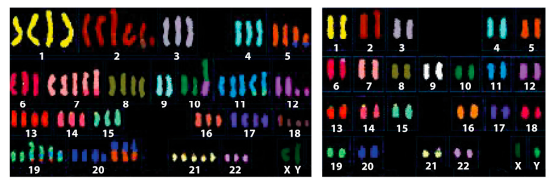
\includegraphics[scale = 1.4]{graphics/chromosomes.png}
                        \caption{\ref{fig:chromosomes}. \small A karyotype of cancer cells of relatively stable genome (Alberts, \emph{et al.}, Molecular Biology of the cell), right.}
                        \label{fig:chromosomes}
					\end{figure}
                        \end{wrapfigure} 
                        We analyze gene expression data to discover pairs of genes that show correlations using a computational approach. 

                    \emph{This project presents:}
				\begin{itemize}
					%\item Cancers are often a result of genomic instability.
					\item A focus on genes suppressing genome instability (GIS genes) since function or expression may often be altered in cancer.
					\item  A computational method to determine normalizing factors that make it possible to discover pairs of GIS genes which show consistent correlation.
					\item Normalizing factors, created by a selection of housekeeping genes (relatively uniform expression across multiple tissues) providing ability to compare gene expressions data and to treat these values by linear regression.
				\end{itemize}

                    \vspace*{6mm}
                \end{block}
			\end{column}
		\end{columns}

%%%%%%%%%%%%%%%%%%%%%%%%%%%%%%%%%%%%%%%%%%%%%%%%%%%%%%%%%%%%%%%%%%%%%

		\begin{columns}

%%%%%%%%%%%%%%%%%%%%%%%%%%%%%%%%%%%%%%%%%%%%%%%%%%%%%%%%%%%%%%%%%%%%%
%
% Left column - Context
%
%%%%%%%%%%%%%%%%%%%%%%%%%%%%%%%%%%%%%%%%%%%%%%%%%%%%%%%%%%%%%%%%%%%%%
            \begin{column}{.5\linewidth}
%%%%%%%%%%%%%%%%%%%%%%%%%%%%%%%%%%%
%
% Method
%
%%%%%%%%%%%%%%%%%%%%%%%%%%%%%%%%%%%
			\begin{block}{\textsc{\textbf{Gene Correlation}}}
				\vspace*{3mm}
%                  \begin{wrapfigure}{r}{0.5\textwidth}
				\begin{figure}
					\centering
					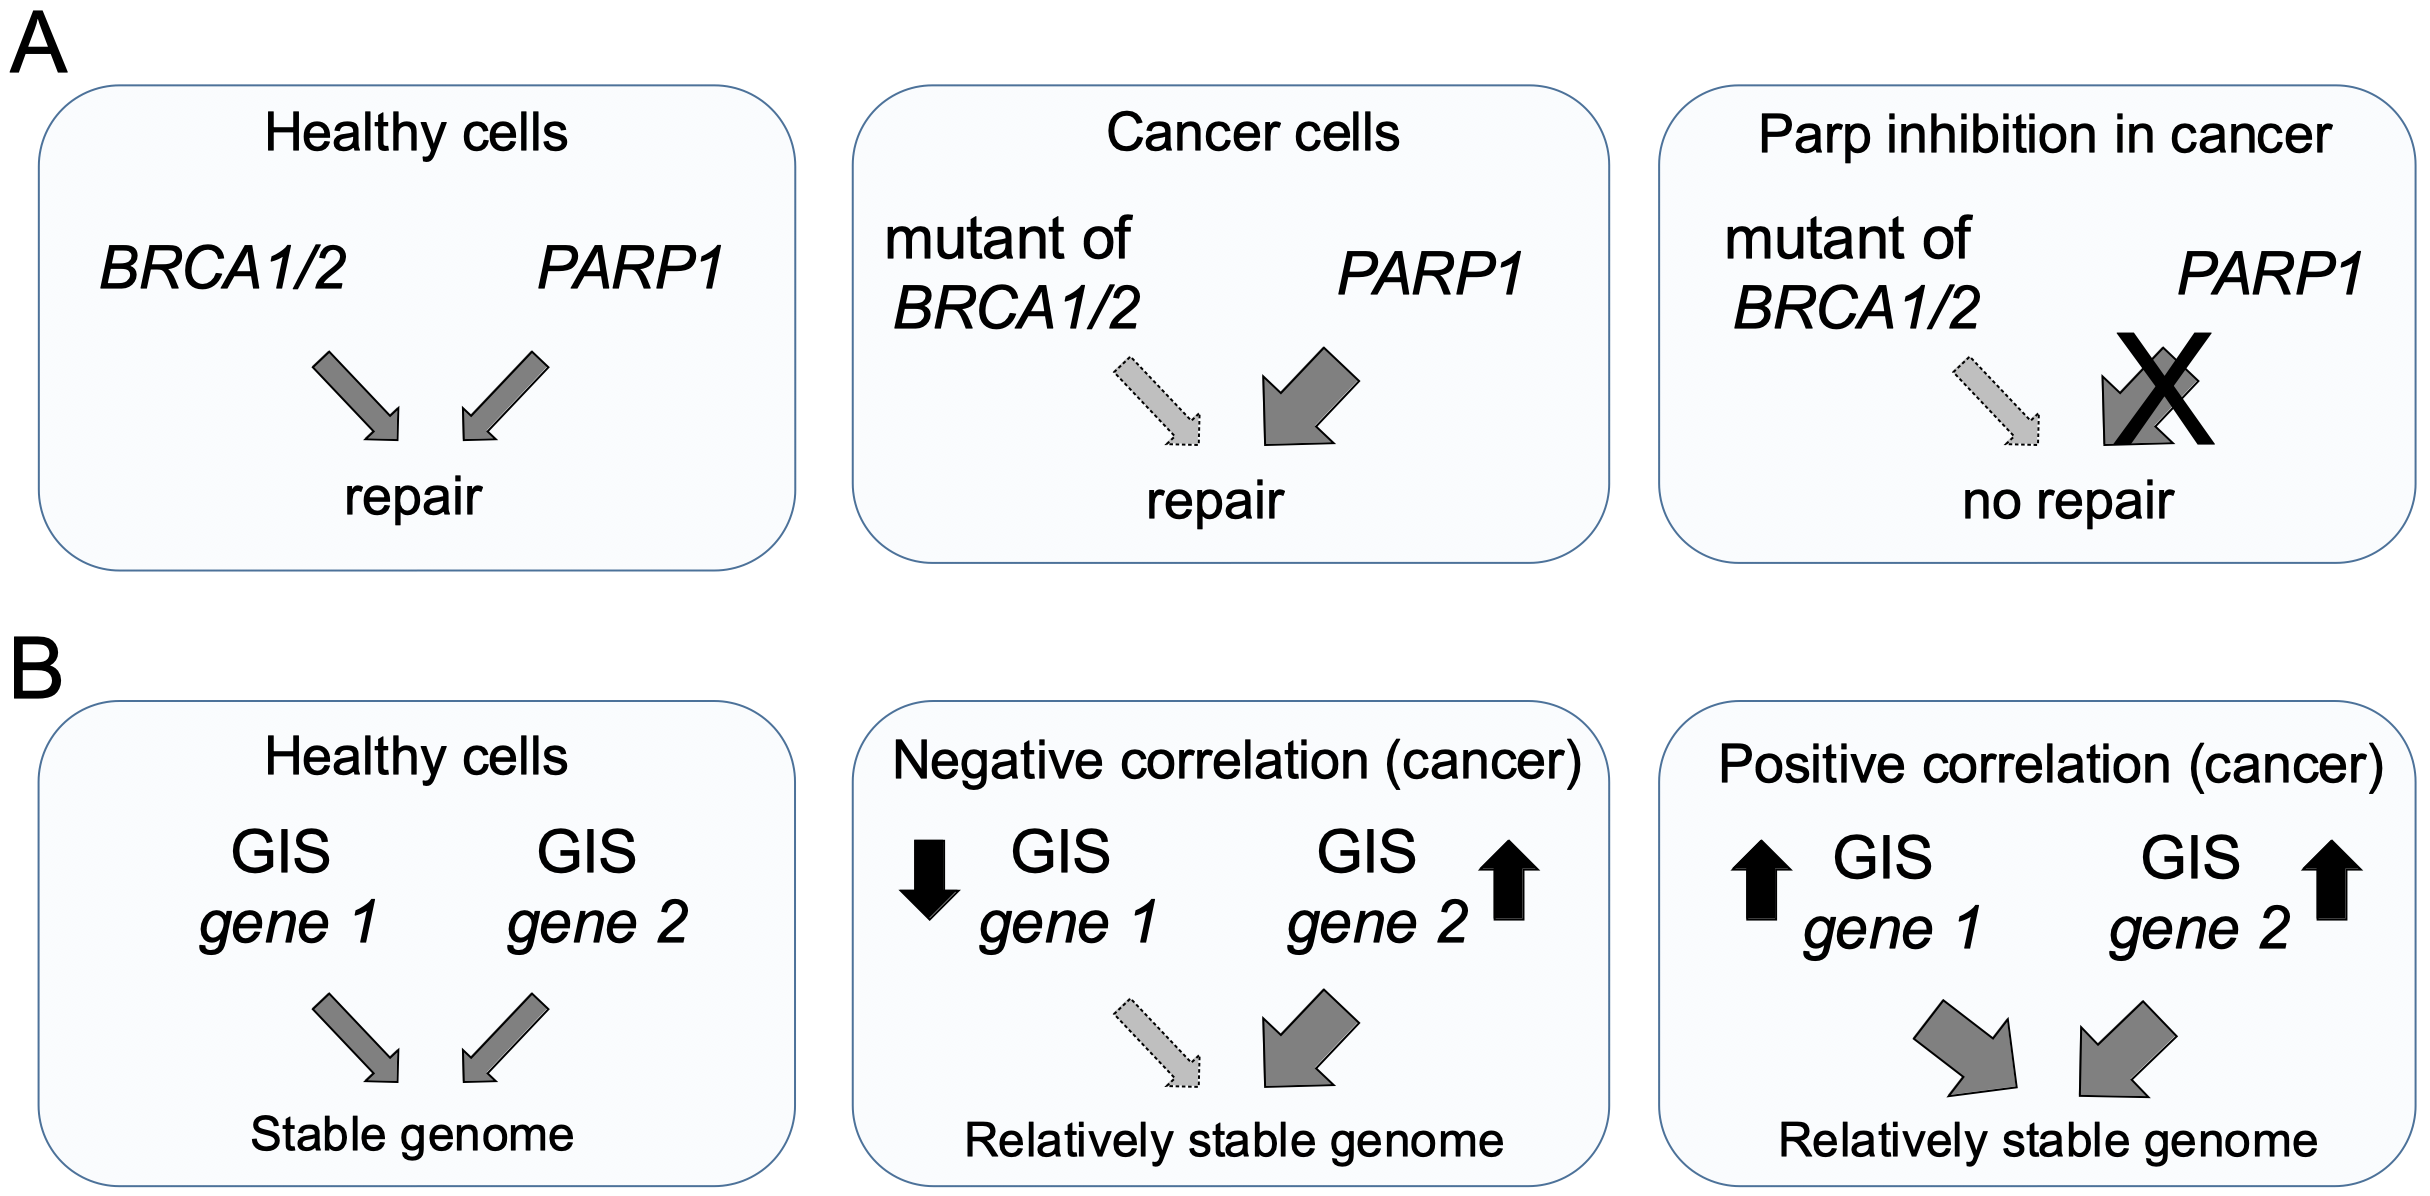
\includegraphics[scale = 0.6]{graphics/braca.png}
					\caption{\ref{fig:braca}. Co-Dependance by genes}
					\label{fig:braca}
%                  \end{wrapfigure}
					\end{figure}
Genetic interactions between genes are often responsible for DNA repair or genome stability.

				\begin{itemize}
					\item FPKM datasets are used to determine the existence of a positive or negative correlation between the expression of two given GIS (suppress genome instability) genes in cancer, Shown in Figure \ref{fig:braca}.
					\item Correlations can reveal if two GIS genes coordinate or if an alteration in the expression of one GIS gene increases dependency of cancer cells on another GIS gene.
				\end{itemize}
				\vspace*{3mm}
			\end{block}
%%%%%%%%%%%%%%%%%%%%%%%%%%%%%%%%%%%
%
% Design
%
%%%%%%%%%%%%%%%%%%%%%%%%%%%%%%%%%%%

  %%%%%
\omitit{                    

			\begin{block}{\textsc{\textbf{Data}}}
				\vspace*{3mm}
%                  \begin{wrapfigure}{r}{0.5\textwidth}
%				\begin{figure}
%					\centering
%					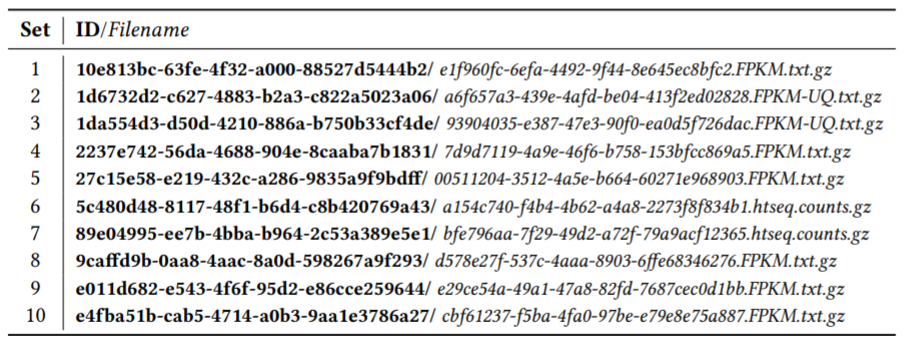
\includegraphics[scale = 2.0]{graphics/dataTable.png}
%					\caption{\ref{fig:dataTable.png}. The de-identified data of our study}
%					\label{fig:dataTable.png}
%                  \end{wrapfigure}
%				\end{figure}

				\begin{itemize}
					\item Genomic Data Commons Data Portal (National Cancer Institute).
					\item \textbf{Proof of concept:} Random selection of ten data sets of breast cancer gene expression. 
					\item Selected subset of genes limited search space, were specific to breast cancer research and reduced noise in results.
					\item Computational approach allows for scalability in gene correlation research.
				\end{itemize}
				\vspace*{3mm}
			\end{block}

}% end of omitit{}

			\begin{block}{\textsc{\textbf{Method: Proof of concept}}}
			\begin{center}
 Random selection of ten data sets of breast cancer gene expression. 
				\begin{figure}
					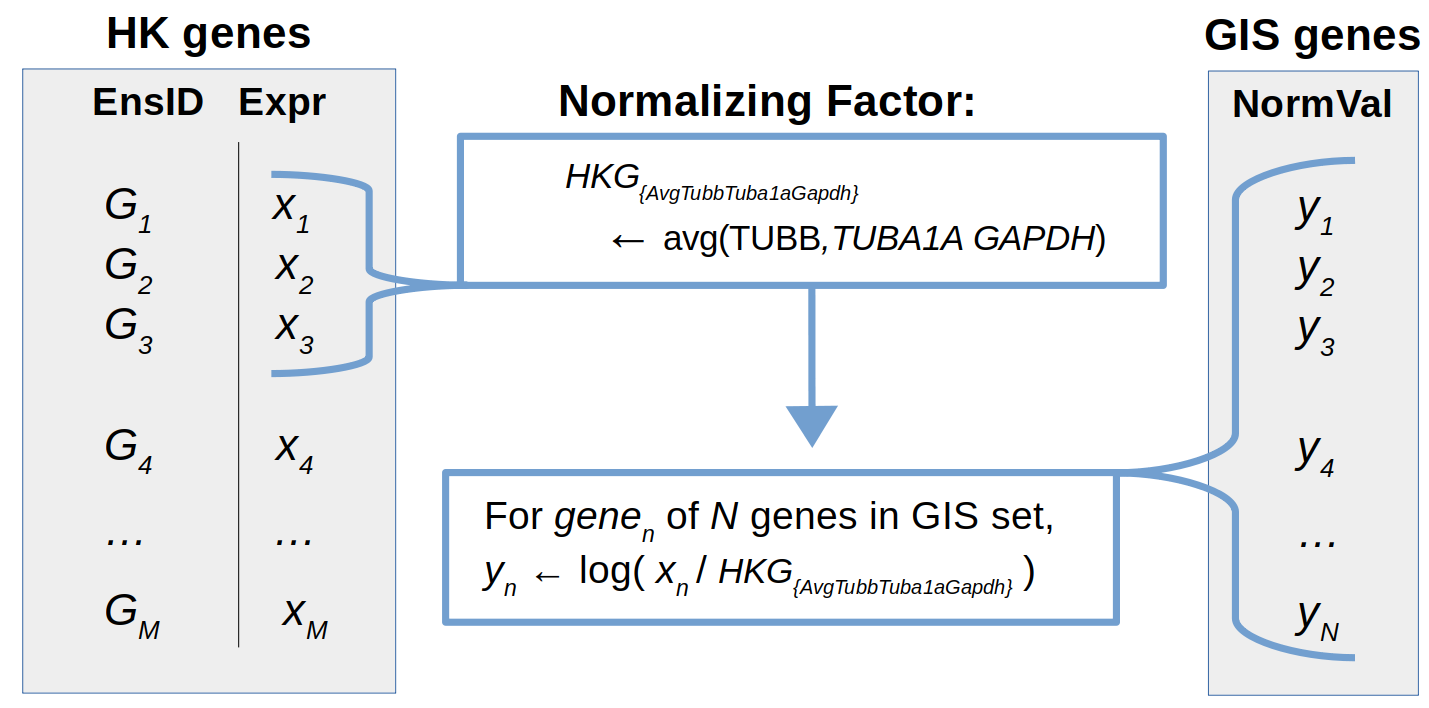
\includegraphics[scale = 0.60]{graphics/normFactor.png}
					\caption{\ref{fig:normFactor}. Determining the normalizing factors}
					\label{fig:normFactor}
				\end{figure}
				
				\begin{center}\end{center} % separation space between both figures
				
				\begin{figure}
					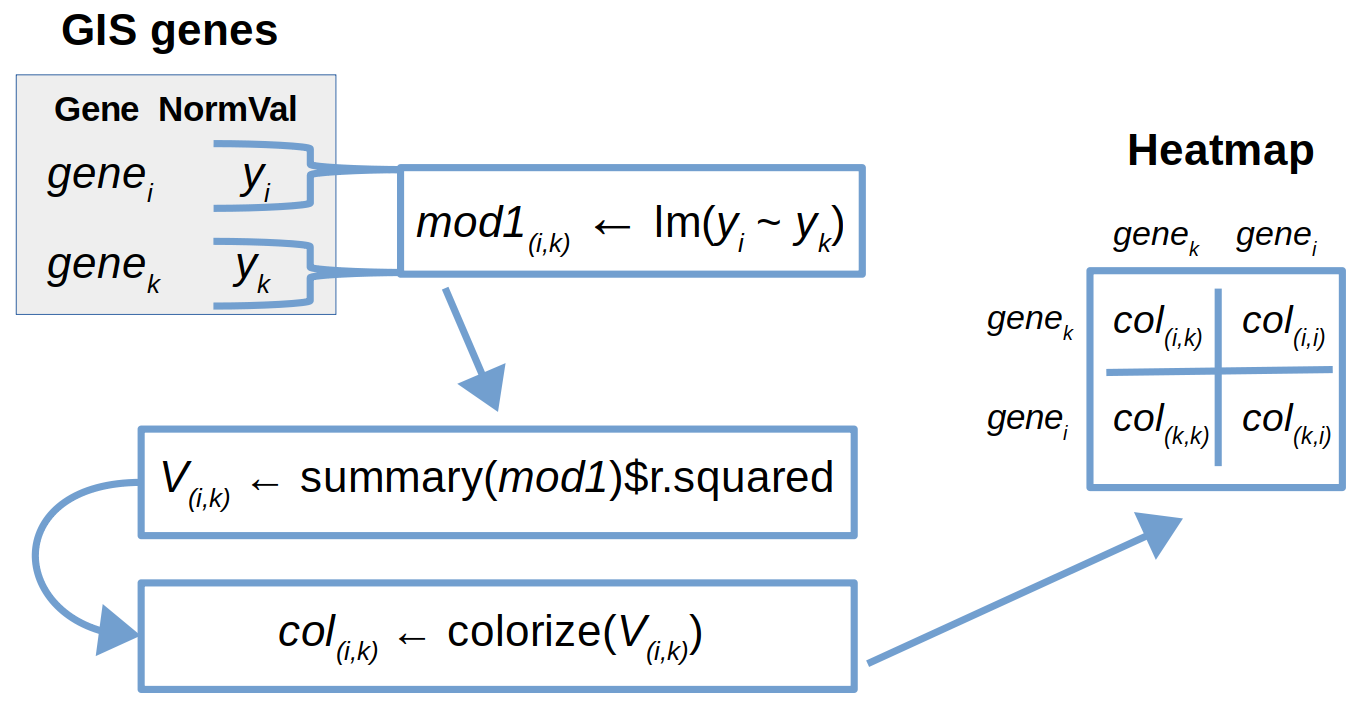
\includegraphics[scale = 0.60]{graphics/lm.png}
					\caption{\ref{fig:lm}. HouseKeeping genes to normalize data sets}
					\label{fig:lm}
				\end{figure}
			\end{center}

				\begin{itemize}
					\item Genomic Data Commons Data Portal (National Cancer Institute).
					\item Selected subset of genes limited search space, were specific to breast cancer research and reduced noise in results.
					%\item Normalizing gene expressions: Expressions of selected GIS genes to normalize genes (WHAT GENES?)
					
				\end{itemize}
			\vspace*{3mm}
                \end{block}
	\end{column}

%%%%%%%%%%%%%%%%%%%%%%%%%%%%%%%%%%%%%%%%%%%%%%%%%%%%%%%%%%%%%%%%%%%%%
%
% Right column - Outcomes
%
%%%%%%%%%%%%%%%%%%%%%%%%%%%%%%%%%%%%%%%%%%%%%%%%%%%%%%%%%%%%%%%%%%%%%
	\begin{column}{.5\linewidth}
%%%%%%%%%%%%%%%%%%%%%%%%%%%%%%%%%%%
%
%
%
%%%%%%%%%%%%%%%%%%%%%%%%%%%%%%%%%%%

%			\begin{block}{\textsc{\textbf{Determining Normalization Factors}}}
%
%
%			\begin{center}
%				\begin{figure}
%					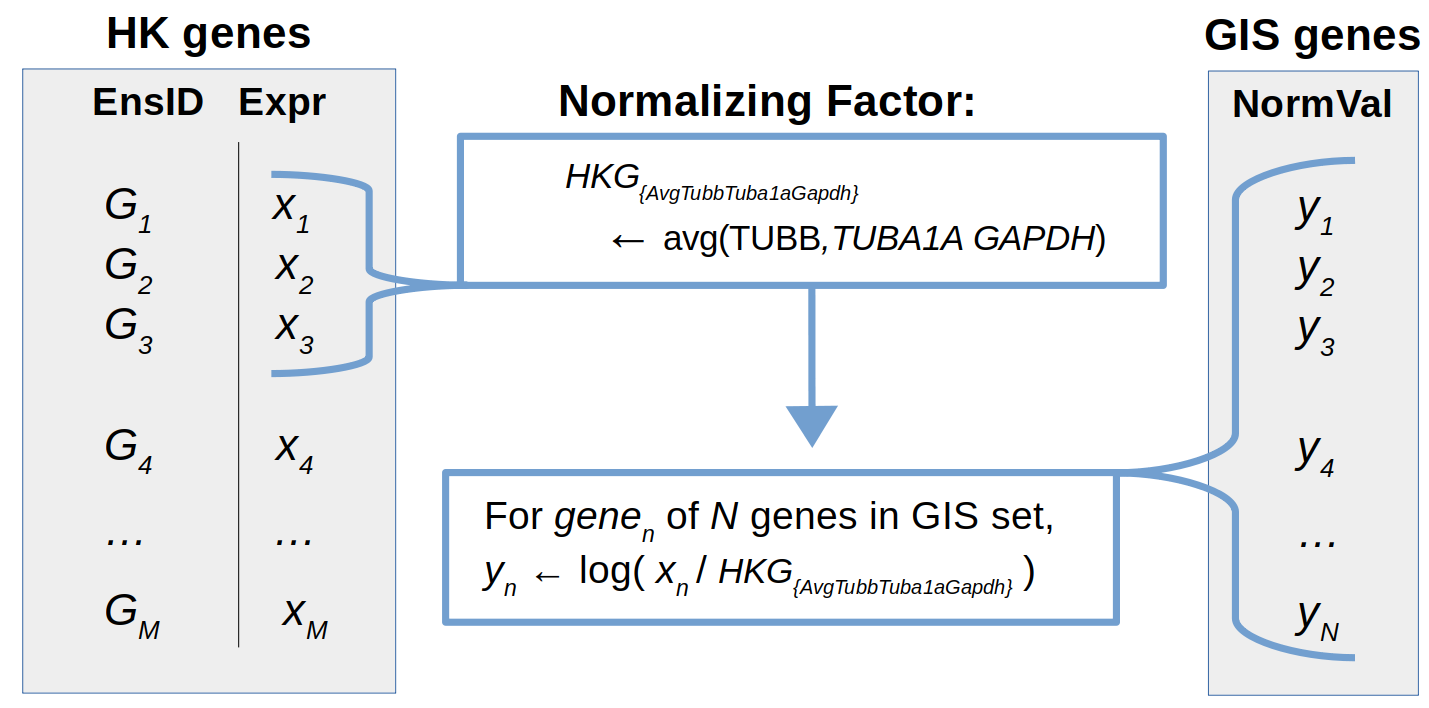
\includegraphics[scale = 0.6]{graphics/normFactor.png}
%					\caption{\ref{fig:normFactor}. Determining the normalizing factors}
%					\label{fig:normFactor}
%				\end{figure}
%			\end{center}
%			\begin{itemize}
%					\item bla bla
%					\item bla bla
%			\end{itemize}
%			\end{block}

		\begin{block}{\textsc{\textbf{R-Squared Values from Linear Models}}}
			\vspace*{3mm}
			\begin{figure}
				\begin{tabular}{cc}
					\hspace*{5mm}

					\includegraphics[scale = 0.28]{graphics/R_geneExpression_A.png}
					\textbf{A.}
					&                     
					\includegraphics[scale = 0.28]{graphics/R_geneExpression_B.png}
					\textbf{B.}\\

					\includegraphics[scale = 0.28]{graphics/R_geneExpression_avgABC.png}
					\textbf{C.}
					&                      
					\includegraphics[scale = 0.32]{graphics/R_geneExpression_AVGG1.png}
					\textbf{D.}\\

					\includegraphics[scale = 0.28]{graphics/R_geneExpression_AVGG2.png}
					\textbf{E.}
					&                      
					\includegraphics[scale = 0.28]{graphics/R_geneExpression_AVGG3.png}
					\textbf{F.}\\
				\end{tabular}				
				\caption{\ref{tab:ge}. Heatmaps of R$^{2}$ values, derived from normalizing factors}
				\label{tab:ge}
			\end{figure}
			\begin{itemize}
				\item $R^{2}$ values in heatmaps from linear regression models, \emph{all-against-all} regressions of GIS genes.

				\item Left to right, R$^{2}$ values, derived from single housekeeping genes to create normalizing factors; $HKG_{Tubb}$, $HKG_{Tuba1a}$, $HKG_{Tubb}$, $HKG_{AvgTubbTuba1aGapdh}$, see Figure 5,\{\textbf{A} - \textbf{C}\}, resp.
				\item Ten housekeeping genes: $HKG_{AvgG1}$,  $HKG_{AvgG3}$,  $HKG_{AvgG3}$, See Figure 5,\{\textbf{D} - \textbf{F}\}, resp.
			\end{itemize}
			\vspace*{3mm}
		\end{block}
                %%%%%%%%%%%%%%%%%%%%%%%%%%%%%%%%%%%
                %
                % Sensors
                %
                %%%%%%%%%%%%%%%%%%%%%%%%%%%%%%%%%%%
		\begin{block}{\textsc{\textbf{Results}}}
			\vspace*{3mm}
			
%			\begin{wrapfigure}{l}{0.47\textwidth}
%				\centering
%				\includegraphics[width=0.35\textwidth]{assets/sensors.jpg}
%				\caption{Arduino board and sensors}
%			\end{wrapfigure}
			
			\begin{itemize}
				\item $HKG_{Tuba1a}$ (\textbf{B}): high diversity of $R^{2}$ values indicated poor normalizing, biologically improbable.
				\item According to regression model results, normalizing factors that were created from larger groups of housekeeping gene produced correlations implying more biological relevance.
			\end{itemize}
			\vspace*{3mm}
	\end{block}

%%%%%%%%%%%%%%%%%%%%%%%%%%%%%%%%%%%
%
% Results
%
%%%%%%%%%%%%%%%%%%%%%%%%%%%%%%%%%%%
	\begin{block}{\textsc{\textbf{Conclusions}}}
		\vspace*{3mm}

		\begin{itemize}
				\item Our results (examples shown in heatmaps of Figure \ref{tab:ge}) indicate normalized data and contain biologically probable findings.
                    	\item \textbf{Single Expression Normalization}:  Normalizing factors derived from single housekeeping genes did not provide generally consistent correlations that were biologically probable.
				\item \textbf{Multiple Expression Normalization}: Using the averaged expression values of multiple housekeeping genes was an effective approach to finding biologically relevant consistency across our data sets.
			\item Our method enabled us to identify the co-expression of gene pairs in breast cancer tissues and compared diverse normalization factors.
			\item Our study also allows reproducibility across data sets and allows for scalability in gene correlation research. 
		\end{itemize}
%		\begin{figure}
%			\includegraphics[scale = 2.5]{}
%			\caption{}
%			\end{figure}
		\vspace*{3mm}
	\end{block}
	\end{column}


	\end{columns}
	\end{frame}
\end{document}









%%%%%%%%%%%%%%%%%%%%%%%%%%%%%%%%%%%%
% Junk bin
% Do not delete the following code, but remove it from the project
%%%%%%%%%%%%%%%%%%%%%%%%%%%%%%%%%%%%






\begin{table}[h!]
\caption{The gene expression data downloaded from the GDC Data Portal available from NCI. The ID and the data set make up the directory and filename of the data set (i.e., {\tt ID/data set.ext}.) In this work, each set is labeled by the index $d$, for $1 \leq d \leq 10$.}
\label{tab:datasets1}
\begin{tabular}{c|l}
\toprule
\textbf{Set} & \textbf{ID}/\emph{Filename}\\
\midrule
1	&	\small \textbf{10e813bc-63fe-4f32-a000-88527d5444b2/}
\emph{e1f960fc-6efa-4492-9f44-8e645ec8bfc2.FPKM.txt.gz} \\
2	&	\small\textbf{1d6732d2-c627-4883-b2a3-c822a5023a06/}
\emph{a6f657a3-439e-4afd-be04-413f2ed02828.FPKM-UQ.txt.gz}\\
3	&	\small\textbf{1da554d3-d50d-4210-886a-b750b33cf4de/}
\emph{93904035-e387-47e3-90f0-ea0d5f726dac.FPKM-UQ.txt.gz}\\
4	&	\small\textbf{2237e742-56da-4688-904e-8caaba7b1831/}
\emph{7d9d7119-4a9e-46f6-b758-153bfcc869a5.FPKM.txt.gz}\\
5	&	\small\textbf{27c15e58-e219-432c-a286-9835a9f9bdff/}
\emph{00511204-3512-4a5e-b664-60271e968903.FPKM.txt.gz}\\
6	&	\small\textbf{5c480d48-8117-48f1-b6d4-c8b420769a43/}
\emph{a154c740-f4b4-4b62-a4a8-2273f8f834b1.htseq.counts.gz}\\
7	&	\small\textbf{89e04995-ee7b-4bba-b964-2c53a389e5e1/}
\emph{bfe796aa-7f29-49d2-a72f-79a9acf12365.htseq.counts.gz}\\
8	&	\small\textbf{9caffd9b-0aa8-4aac-8a0d-598267a9f293/}
\emph{d578e27f-537c-4aaa-8903-6ffe68346276.FPKM.txt.gz}\\
9	&	\small\textbf{e011d682-e543-4f6f-95d2-e86cce259644/}
\emph{e29ce54a-49a1-47a8-82fd-7687cec0d1bb.FPKM.txt.gz}\\
10	&	\small\textbf{e4fba51b-cab5-4714-a0b3-9aa1e3786a27/}
\emph{cbf61237-f5ba-4fa0-97be-e79e8e75a887.FPKM.txt.gz}\\	
\bottomrule
\end{tabular}
\end{table}



\begin{table}[h!]
\caption{The legend of variable names of the normalizing factors that were used to normalize the gene expressions. For each set, these variables were created to be used to normalize all expressions of the set.}
\label{tab:legend}
\begin{tabular}{ll}
\toprule
\textbf{Variable}	& \textbf{Expr. in Norm. Fact.}\\
\midrule
$HKG_{Tubb}$ & Single expression of \emph{TUBB}\\
$HKG_{Tuba1a}$ & Single expression of \emph{TUBA1A}\\
$HKG_{Gapdh}$ & Single expression of \emph{GAPDH}\\
\hline
$HKG_{AvgTubbTuba1aGapdh}$ & Avg of three genes\\
\hline
$HKG_{AvgG1}$ & Avg of ten genes in group 1\\
$HKG_{AvgG2}$ & Avg of ten genes in group 2\\
$HKG_{AvgG3}$ & Avg of ten genes in group 3\\

\bottomrule
\end{tabular}
\end{table}



% original sizes of heatmaps

					\includegraphics[scale = 0.30]{graphics/R_geneExpression_A.png}
					\textbf{A.}
					&                     
					\includegraphics[scale = 0.30]{graphics/R_geneExpression_B.png}
					\textbf{B.}\\

					\includegraphics[scale = 0.30]{graphics/R_geneExpression_avgABC.png}
					\textbf{C.}
					&                      
					\includegraphics[scale = 0.34]{graphics/R_geneExpression_AVGG1.png}
					\textbf{D.}\\

					\includegraphics[scale = 0.30]{graphics/R_geneExpression_AVGG2.png}
					\textbf{E.}
					&                      
					\includegraphics[scale = 0.30]{graphics/R_geneExpression_AVGG3.png}
					\textbf{F.}\\
